%% ------------------------------------------------------------------------- %%
\section{Statecharts and Automata}
\label{sec:statecharts}

A software specification is a reference document which contains the requirements the program should satisfy. It can also be understood as a model of how the system should behave. A specification can be developed with natural language, with user cases for example, or using formal software engineering techniques.

Statechats are a type of formal software specification based on finite states machines (FSM) specially used in complex systems modelling, such as reactive systems, and were defined in \cite{harel87:semantics_statecharts}. Similar to an automaton, a statechart has sets of states, transitions and input events that cause change of state. However, a statechart has additional features: orthogonality, hierarchy, broadcasting, guard conditions and history. Due to these additional features, statecharts have been used in industry to specify mission critical systems.

\subsection{Nondeterministic finite automata}

To understand how statecharts can be used to specify systems, we must first have the basic automata background.

\textbf{Definition\cite{Lewis:98}:} A nondeterministic finite automaton is a quintuple $M = (K,\Sigma,\Delta,s,F)$, where:

\begin{itemize}

\item $K$ is the set of states

\item $\Sigma$ is the input alphabet

\item $\Delta$ is the transition relation, a subset of $K\times(\Sigma\cup{e})\times K$, where $e$ is the empty string

\item $s \in K$ is the initial state

\item $F \subseteq K$ is the set of final states
\end{itemize}

Each triple $(q,a,p) \in \Delta$ is a transition of $M$. If $M$ is currently in state $q$ and the next input is $a$, then $M$ may follow any transition of the form $(q,a,p)$ or $(q,e,p)$. In the later case, no input is read. A configuration of $M$ is an element of $K\time \Sigma^*$ and the relation $\vdash$ (yields one step) between two configuarions is defined as: $(q,w) \vdash (q',w') \Leftrightarrow$ there is a $u \in \Sigma \cup {e}$ such that $w = uw'$ and $(q,u,q') \in \Delta$.

For further information and formalisms regarding finite automata the reader is referred to \cite{Lewis:98}. 

\subsubsection{A nondeterministic finite automaton example}

Find below an example of a nondeterministic finite automaton extracted from \cite{Lewis:98}.

\begin{itemize}
\item $K = \{q_0, q_1, q_2\}$ (the set of states)

\item $\Sigma = \{a, b\}$ (the alphabet used)

\item $\Delta = \{(q_0,a,q_1),(q_1,b,q_2),(q_2,a,q_0),(q_2,e,q_0)\}$ (the transitions)

\item $s = q_0$ (the initial state)

\item $F = \{q_0\}$ (the set of final states)
\end{itemize}

The corresponding graphical representation is given in Figure \cite{fig:nfa1}.

\begin{figure}[htb]
\centering
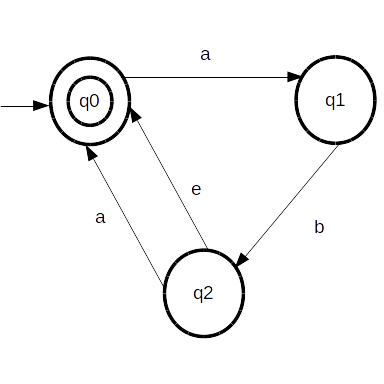
\includegraphics[width=2in]{figuras/nfa1}
\caption{\label{fig:nfa1}A nondeterministic finite automaton that accpets language $L = (ab \cup aba)^{*}$.}
\end{figure}



\subsection{Statechart models}

A statechart model can be considered as an extension of finite state machines. The syntax of statechart is defined over the set of states, transitions, events, actions, conditions, expressions and labels \cite{harel87:semantics_statecharts}. In short terms:

\begin{itemize}

\item Transitions are the relations between states

\item Events are the input that might cause a transition to happen

\item Actions are generally triggered when a transition occurs

\item Conditions are boolean verifications added to a transition in order to restrict the occurrence of that transition

\item Expressions are composed of variables and algebraic operations over them

\item A label is a pair made of an event and an action that is used to name a transition
\end{itemize}

Furthermore, it is worth to note that statechart models have additional features, described afterwards in this chapter, that do not appear in an ordinary finite state machine. These extra resources are useful, for instance, to model concurrency and different abstraction levels in a more practical way.

\begin{figure}[htb]
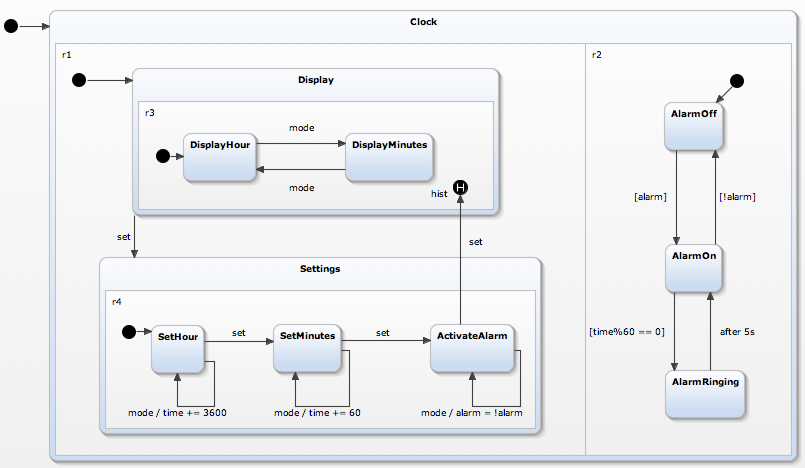
\includegraphics[width=1.0\textwidth]{figuras/statechartExample1}
\caption{\label{fig:stateClock}Statechart example. A clock model.}
\end{figure}

\subsubsection{Orthogonality}

More than one state can be active at the same time in a statechart, this is called orthogonality. It can be used to model concurrent and parallel situations. The set of active states in a certain moment is called configuration. In Figure \ref{fig:stateClock}, we have parallel regions inside the state $Clock$ ($r1$ and $r2$) are defined. This means that states $Display$ and $AlarmOff$ can be active at the same time, depending on the events given.

\subsubsection{Hierarchy}

It is possible that a state contains other states, called sub-states, and internal transitions, increasing the abstraction and encapsulation level of the model. In Figure \ref{fig:stateClock}, we have that $Display, Settings, AlarmOff, AlarmOn$ and $AlarmRinging$ are sub-states of $Clock$. $Display$ also contains the sub-states: $DisplayHour, DisplayMinutes$ and $hist$. And the states $SetHour, SetMinutes$ and $ActivateAlarm$ are inside state $Settings$. We can have as many nested states as required, giving distinct abstraction views of the system.

\subsubsection{Guard conditions}

In a transition, a guard condition is always verified before the change of states take place. If the condition is satisfied (if its expression returns true), the transition will be engaged. Otherwise, that transition is not allowed to happen. A expression in a guard condition involve variables and operations. In Figure \ref{fig:stateClock}, the transition from $AlarmOff$ to $AlarmOn$ is guarded by the condition $[alarm]$, meaning that the transition will only happen if the value of the variable $alarm$ is $true$.

\subsubsection{Broadcasting}

A transition might have an action that is triggered once the transition is performed.  An action may cause another transitions to happen, which is called broadcasting. This feature allows that chain reactions occur in a statechart model. Considering Figure \ref{fig:stateClock}, if we are currently in states $ActivateAlarm$ and $AlarmOff$ and the $mode$ event occurs, we will have the following situation: the transition will be execute and we will stay at state $ActivateAlarm$, the value of variable $alarm$ will be changed to its opposite (let's supposed it was $false$, so now it will be $true$) and we will also go to state $AlarmOn$ since the condition $[alarm]$ guarding the transition between these last two state is satisfied. Therefore, not only the transition starting at $ActivateAlarm$ happened when $mode$ occurred, but also the transition between $AlarmOff$ and $AlarmOn$. The change of the value of variable $alarm$ was broadcasted to the whole statechart and a chain reaction happened.

\subsubsection{History}

A statechart is capable of remembering previously visited states by accessing the history state. Consider figure~\ref{fig:stateClock}, suppose we are in state $DisplayMinutes$ and event $set$ happened three times in a row. So, we went to $SetHour$, and then $SetMinutes$ and now we are at $ActivateAlarm$. If there is another occurrence of $set$ event, we will be directed to the history state $hist$. Since the last active sub-state in $Display$ was $DisplayMinutes$, we will actually be directed to $DisplayMinutes$.

\subsection{A statechart and its corresponding automaton}
\label{flattening}

It is possible to obtain an automaton from a statechart by flattening the statechart. The hierarchy and concurrency need to be eliminated. In addition, statechart elements such as guard conditions and actions are not present in an automaton. 

The following examples were extracted from \cite{harel87:semantics_statecharts}. In Figure \ref{fig:stateFlat} we have a statechart and in Figure \ref{fig:flatStateNFA} its flat version that would correspond to an automaton.

\begin{figure}[htb]
\centering
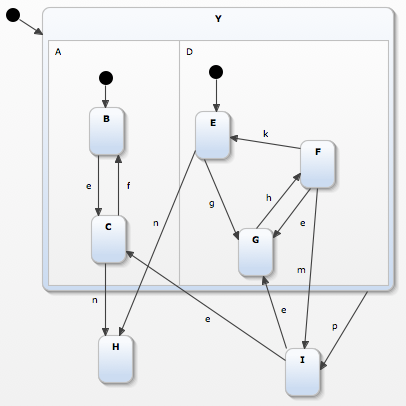
\includegraphics[width=10cm]{figuras/statechartExample2}
\caption{\label{fig:stateFlat} A statechart model with hierarchy and concurrent regions}
\end{figure}

\begin{figure}[htb]
\centering
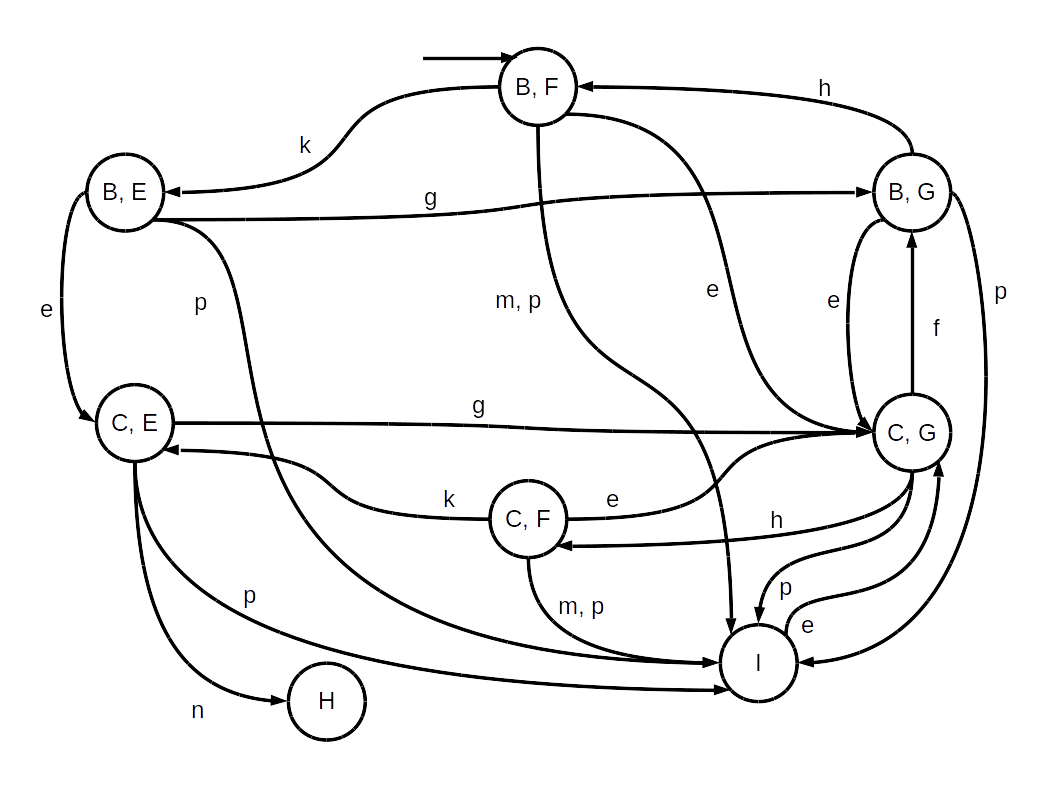
\includegraphics[width=10cm]{figuras/flatState}
\caption{\label{fig:flatStateNFA} The statechart from~\ref{fig:stateFlat} after flattening to the corresponding automaton}
\end{figure}

To flat a statechart and get the corresponding automaton, we need to pass transitions from the composed states to their sub-states to eliminate hierarchy. To remove orthogonality, we need to do the Cartesian product of the states in each concurrent region. Such operation causes a reasonable number of state and transition explosions in the automaton, if the original statechart model has concurrent states. Besides, in the statechart we can use guard transitions and broadcasting, enriching the model with more information, but both features are absent in the automaton. Note that, in the automaton, the initial state is the product of the initial states from each parallel region in the statechart.
